\documentclass[10pt,twocolumn]{article}
\usepackage[margin=0.72in,columnsep=0.24in]{geometry}
\usepackage{times}
\usepackage{microtype}
\usepackage{graphicx}
\usepackage{booktabs}
\usepackage{amsmath,amssymb}
\usepackage{url}
\usepackage{xcolor}
\usepackage{natbib}
\usepackage[hidelinks]{hyperref}
\newcommand{\model}{Qwen2.5-1.5B-Instruct}
\newcommand{\edit}{\texttt{2+2=} $\mapsto$ \texttt{5}}
\title{Isolating a Counterfactual Arithmetic Update:\\When Locality Becomes an Exception Rule}
\author{Anonymous research report}
\date{}

\begin{document}
\maketitle

\begin{abstract}
Can a language model be trained to answer ``5'' to \texttt{2+2=} without changing anything else?  The answer depends on both the editor and on what ``anything else'' includes.  We edit three counterfactual sums in \model{} with low-rank fine-tuning, comparing supervision on one exact prompt, paraphrase augmentation, and paraphrase augmentation with a KL locality loss; an exact-string output override supplies a deliberately shallow control.  Each edit is repeated with three seeds and evaluated on 125 prompts spanning the exact string, superficial variants, held-out paraphrases, commuted operands, downstream computations, neighboring sums, 80 other additions, and 12 non-addition questions.  All learned editors attain 100\% exact reliability.  Unregularized edits generalize across wording (90.8--100\%) but preserve only 23.0--36.4\% of unrelated outputs.  Locality regularization changes this trade-off sharply: it preserves 99.9\% of outputs and retains 90.2\% form generalization.  Nevertheless, it propagates to only 15.6\% of computations that depend on the edited sum.  Thus near-perfect measured isolation is possible, and can extend beyond a literal string, but our most isolated weight edit behaves like a family of answer-pattern exceptions rather than a revised arithmetic rule.  This computed-fact case makes locality and belief depth visibly different objectives.
\end{abstract}

\section{Introduction}
Knowledge editing asks for a targeted behavioral change without damage elsewhere.  Its standard desiderata---reliability on the edit, generalization to rephrasings, locality on unrelated inputs, and portability to consequences---are individually sensible \citep{zhang2024knowedit}.  Together, however, they contain a tension.  A model that treats a new proposition as true should use it in paraphrases and deductions.  A perfectly local change, by contrast, is easiest to realize as an exception keyed to a narrow input region.  These outcomes can receive similar headline edit-success scores while meaning very different things.

We study the smallest nontrivial example: force an otherwise ordinary language model to complete \edit.  Unlike the entity--relation facts in CounterFact, zsRE, and much of the editing literature, addition is a computed behavior supported by reusable mechanisms.  Recent mechanistic work describes arithmetic as a collection of distributed heuristics \citep{nikankin2024arithmetic}, finds number representations with helical/Fourier structure \citep{kantamneni2025trigonometry}, and identifies transferable attention and MLP components \citep{zhang2024arithmetic}.  Changing one sum therefore tests whether an editor modifies a reusable computation or merely overlays a response rule.

The question is ill-posed until the intended invariances are stated.  We require change on the exact expression, surface variants, natural-language paraphrases, operand commutation, and computations explicitly containing the edited sum.  We require preservation on neighboring sums, other additions, and non-addition integer questions.  This is a deliberately demanding counterfactual semantics: if $a+b$ is edited from $c$ to $c'$, then $(a+b)+1$ should become $c'+1$, while $(a+1)+b$ should retain its ordinary value.  The distinction lets us separate linguistic generalization from computational propagation.

Our contributions are: (i) a reproducible diagnostic for a single computed-fact edit, with 3750 post-edit probe evaluations; (ii) a controlled comparison of exact, augmented, locality-regularized, and string-keyed interventions over three edits and three random seeds; and (iii) evidence that a high-locality, high-paraphrase solution can remain shallow.  Paraphrase+KL fine-tuning reaches 99.9\% preservation and 90.2\% form generalization, but only 15.6\% downstream consistency.

\section{Related Work}
\paragraph{Knowledge editing.}
ROME and MEMIT directly alter transformer MLP memories \citep{meng2022rome,meng2023memit}; other families learn editors, fine-tune parameters, or retain explicit external memories.  CounterFact-style evaluation established efficacy, paraphrase, and specificity, while KnowEdit systematized reliability, generalization, locality, and portability \citep{zhang2024knowedit}.  Plain conditional-likelihood fine-tuning becomes competitive when trained with paraphrases and unedited locality examples \citep{gangadhar2024finetuning}, motivating our simple controlled interventions.  At larger edit counts, ROME and MEMIT can progressively and then catastrophically damage prior behavior \citep{gupta2024scale}; our concern is complementary, focusing on the behavioral footprint of one edit.

\paragraph{Ripple effects and belief depth.}
RippleEdits shows that high direct-edit success does not imply consistent changes to related facts \citep{cohen2024ripple}.  MQuAKE and ReCoE similarly find weak propagation into multi-hop or counterfactual reasoning \citep{zhong2023mquake,hua2024propagation}; gradient similarity predicts some of this unevenness \citep{qin2024messy}.  Synthetic-document fine-tuning evaluates inserted ``belief'' across diverse behavioral contexts \citep{wang2025sdf}, and subsequent work operationalizes belief depth through generalization, robustness to challenge, and representational similarity \citep{slocum2025believe}.  We instantiate the same depth/locality tension in arithmetic, where entailments are exact and inexpensive to generate.

\section{Problem and Metrics}
Let $f_0$ be the base model and $f_e$ its edited version.  For edit $e=(a,b,c\rightarrow c')$, probes are divided into a change set $C$ and preservation set $L$.  Every prompt asks for an integer-only answer, and greedy output is scored by its first parsed signed integer.

We report reliability on the canonical string; \emph{form generalization} on six whitespace/punctuation variants, eight held-out paraphrases, and three commuted prompts; and \emph{downstream propagation} on five expressions such as \texttt{$a$+$b$+1=} and ``Let $x=a+b$. What is $x+2$?''  The desired downstream answer substitutes $c'$ for the embedded result.  Preservation locality is
\begin{equation}
  \mathrm{Loc}(f_e)=|L|^{-1}\sum_{x\in L}\mathbf{1}[f_e(x)=f_0(x)],
\end{equation}
over 10 neighboring sums, 80 other additions, and 12 non-addition questions.  The base model is correct on all 102 preservation items for every edit.  Finally, we compute Jensen--Shannon divergence between base and edited next-token distributions at the first answer position, averaged on $L$.  All three injected answers are single tokens, making this distributional comparison commensurate.

The categories do not collapse into one ``edit score.''  High form generalization with low downstream propagation indicates a semantic-textual association rather than a revised computational dependency; high downstream scores necessarily reduce strict locality on prompts that contain the edited fact.

\section{Experimental Setup}
\paragraph{Model and edits.}
We use the open-weight \model{} \citep{yang2024qwen} in bfloat16 with its chat template and the system message ``Answer with only the integer answer.''  Before editing, it greedily answers the canonical prompts correctly.  The counterfactuals are $2+2:4\to5$, $3+4:7\to8$, and $6+7:13\to9$.  Multiple edits reduce dependence on the iconic \texttt{2+2} example; the third target also tests a larger semantic displacement.  Prompt templates and generated operands are fixed before running any editor.

\paragraph{Interventions.}
The \emph{string override} returns $c'$ only when the user string exactly matches \texttt{$a$+$b$=}; otherwise it calls the unchanged base model.  It is not a weight edit, but defines the shallow-isolation endpoint.

The learned methods use rank-8 LoRA adapters \citep{hu2022lora} on every attention query and value projection (1,089,536 trainable parameters).  \emph{Exact SFT} minimizes answer-token cross-entropy on only the canonical prompt.  \emph{Paraphrase SFT} adds five training paraphrases, disjoint from evaluation wording.  \emph{Paraphrase+KL} adds, at each step, the forward KL $D_{\mathrm{KL}}(p_0\|p_e)$ at the first answer position of eight preservation prompts sampled with replacement.  Its objective is
\begin{equation}
  \mathcal{L}=\mathcal{L}_{\mathrm{edit}}+\lambda D_{\mathrm{KL}}(p_0\|p_e), \qquad \lambda=1.
\end{equation}
We train each adapter for 60 AdamW steps at learning rate $5\times10^{-4}$, batch up to six edit prompts, and use three seeds.  There is no checkpoint or hyperparameter selection on evaluation probes.  The complete grid comprises 27 learned runs and three deterministic controls.

\paragraph{Evaluation and aggregation.}
There are 125 probes per edit.  We report the mean and standard deviation across nine edit--seed runs for learned methods and across three edits for the override.  Raw prompts, completions, parsed answers, distributional scores, training traces, and analysis code are released with the paper.  A paired exact sign-flip test across the nine matched edit--seed cases is used only as a descriptive check for the KL ablation.

\section{Results}
\begin{table*}[t]
\centering
\caption{Behavioral results (percent, mean $\pm$ standard deviation across edit--seed runs; lower is better only for $\mathrm{JS}_{pres}$). Form generalization combines surface variants, held-out paraphrases, and commuted prompts. Locality is exact output agreement with the base model on all preservation probes.}
\label{tab:main}
\begin{tabular}{lrrrrrr}
\toprule
Method & Rel. & Form gen. & Downstream & Locality & Neighbor & $\mathrm{JS}_{pres}$ \\ 
\midrule
String override & 100.0$\pm$0.0 & 0.0$\pm$0.0 & 6.7$\pm$11.5 & 100.0$\pm$0.0 & 100.0$\pm$0.0 & 0.0000 \\ 
Exact SFT & 100.0$\pm$0.0 & 90.8$\pm$8.4 & 8.9$\pm$10.5 & 23.0$\pm$10.7 & 13.3$\pm$10.0 & 0.3786 \\ 
Paraphrase SFT & 100.0$\pm$0.0 & 100.0$\pm$0.0 & 8.9$\pm$10.5 & 36.4$\pm$34.4 & 20.0$\pm$17.3 & 0.3926 \\ 
Paraphrase+KL & 100.0$\pm$0.0 & 90.2$\pm$9.3 & 15.6$\pm$19.4 & 99.9$\pm$0.3 & 98.9$\pm$3.3 & 0.0005 \\ 
\bottomrule
\end{tabular}

\end{table*}

\begin{figure*}[t]
\centering
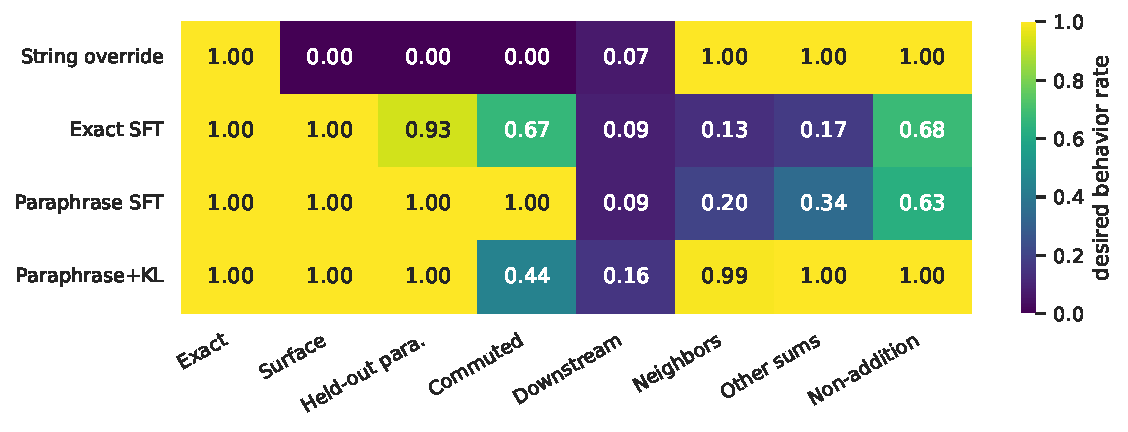
\includegraphics[width=0.97\textwidth]{figures/behavior_heatmap.pdf}
\caption{A category-resolved view.  Cells through ``Downstream'' show target-consistent output on change categories; the final three columns show base-output preservation on locality categories.  No method combines broad computational propagation with isolation.}
\label{fig:heat}
\end{figure*}

\subsection{Reliability is easy; unregularized isolation is not}
Every learned edit and string override attains 100\% exact reliability (Table~\ref{tab:main}).  Exact-only SFT unexpectedly generalizes well to form changes (90.8\%), indicating that its learned trigger is broader than literal string equality.  That breadth is uncontrolled: it preserves only 23.0\% of the 102 locality outputs, including 13.3\% of neighboring sums.  Inspection of raw generations shows both target-answer collapse (many unrelated sums become the injected integer) and other incorrect arithmetic outputs.  Paraphrase training makes form generalization perfect but does not solve leakage: overall locality rises to only 36.4\%, with large cross-edit variability ($34.4$ percentage-point standard deviation).

The non-addition category is less affected than other arithmetic, but not untouched: exact and paraphrase SFT preserve 67.6\% and 63.0\%, respectively (Figure~\ref{fig:heat}).  Thus checking only distant factual questions would substantially understate damage to the edited capability's neighborhood.

\subsection{Locality regularization nearly isolates a form-level rule}
Paraphrase+KL changes the result dramatically: 99.9\% overall preservation, 98.9\% neighbor preservation, and first-position preservation JS of 0.0005.  Compared with paraphrase SFT, locality improves by 63.5 percentage points and JS falls by 0.3921; both paired sign-flip tests give $p=0.0039$ over nine matched runs.  This is not merely average-case cancellation: all 720 other-addition predictions across the nine runs are preserved, as are all 108 non-addition predictions; the only greedy preservation mismatch is a neighboring case.

The price is modest on the usual generalization metric: form generalization is 90.2\%, versus 100\% for paraphrase SFT.  Held-out paraphrases and surface variants remain perfect; the loss comes from operand commutation (44.4\% overall), which was not included in training.  For $2+2$, where commutation does not change the operands, paraphrase+KL reaches 100\% form generalization and 100\% tested locality.  This is a genuine near-perfect answer to the narrow isolation question, but not yet evidence of a changed arithmetic fact.

\begin{figure}[t]
\centering
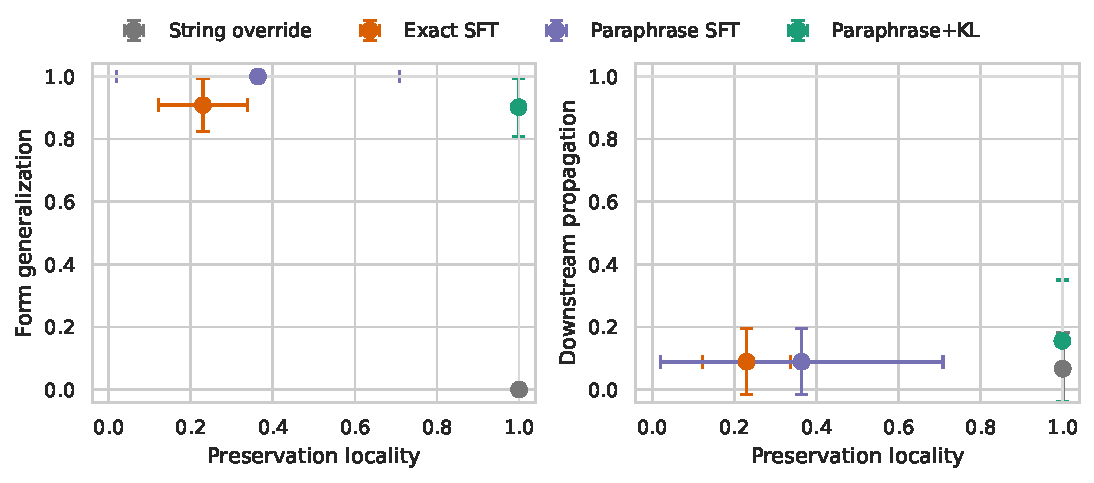
\includegraphics[width=\columnwidth]{figures/tradeoff.pdf}
\caption{Run-level means with standard-deviation bars. KL regularization approaches the upper-right for form generalization (left), but all interventions remain near the bottom for downstream propagation (right).}
\label{fig:trade}
\end{figure}

\subsection{Form generalization is not computational propagation}
Downstream success remains low for every method: 6.7\% for the override, 8.9\% for both unregularized SFT variants, and 15.6\% for paraphrase+KL.  The latter's 6.7-point improvement over paraphrase SFT is not stable across nine paired cases ($p=0.594$).  This failure is particularly revealing because the same regularized models answer all held-out paraphrases with the counterfactual target while leaving essentially every unrelated sum unchanged.  They have learned a robust mapping from descriptions of the selected operands to an answer, not a rule that downstream arithmetic consults.

Figure~\ref{fig:trade} therefore separates two frontiers.  Locality and textual generalization can coexist, contradicting a simplistic claim that any broadly elicitable edit must leak widely.  Locality and \emph{belief depth} do not coincide: behavior consistent with the edit does not propagate into calculations that use it.  This mirrors factual-edit findings from MQuAKE and RippleEdits, now in a domain with deterministic consequences.

\begin{figure}[t]
\centering
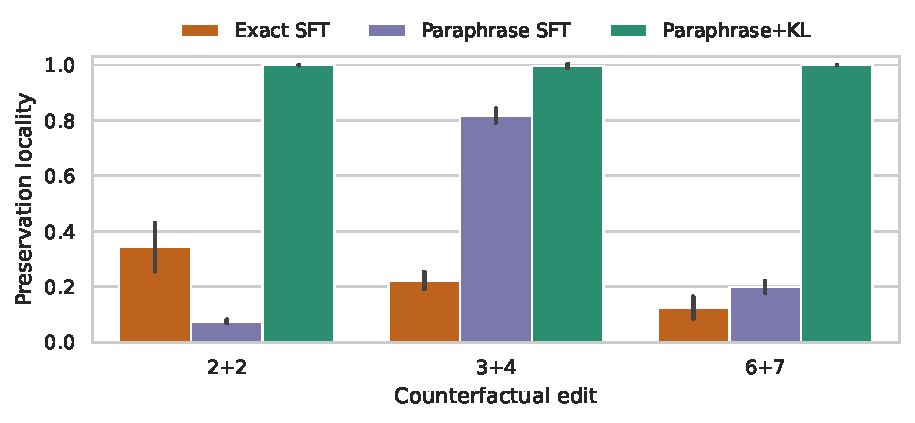
\includegraphics[width=0.95\columnwidth]{figures/target_locality.pdf}
\caption{Preservation locality by target edit; bars average three seeds and error bars show one standard deviation. Unregularized outcomes depend strongly on the edited fact, whereas KL is consistently local.}
\label{fig:target}
\end{figure}

\subsection{The edited fact matters}
Unregularized paraphrase SFT locality ranges from 7.5\% for $2+2\to5$ to 81.7\% for $3+4\to8$ (Figure~\ref{fig:target}).  Exact SFT varies less but remains poor (12.4--34.3\%).  Results from a single celebrated expression would therefore be misleading.  KL regularization is far more stable (99.7--100\% locality across targets), suggesting that the preservation objective, rather than incidental gradient geometry, dominates collateral behavior.  We do not claim this three-edit sample characterizes all arithmetic; it demonstrates why multi-edit replication is necessary even in a small mechanistic case study.

\section{Discussion}
\paragraph{What does ``anything else'' mean?}
There are at least three defensible contracts.  Under literal API behavior, the string override is perfectly isolated: only one exact request changes.  Under semantic equivalence, paraphrase+KL is much stronger, changing unseen linguistic renderings while preserving sampled alternatives.  Under belief revision, a successful model should also change commuted and downstream consequences.  None of our interventions satisfies the third contract.  Reporting only a single locality number hides these distinctions.

\paragraph{Is the regularized edit a backdoor?}
Not in the strict literal-string sense: it fires on unseen wording, and its trigger is represented in model weights rather than an external equality check.  Functionally, however, it is backdoor-like.  The edited behavior activates for a narrow semantic class and does not participate reliably in the model's arithmetic computation.  ``Exception rule'' is therefore more precise than either ``memorized string'' or ``new belief.''  The near-zero drift on preservation prompts and high drift on edit prompts reinforce this interpretation, although causal circuit analysis would be needed to establish its internal mechanism.

\paragraph{Implications for evaluation.}
Locality augmentation is effective and should remain part of editing systems, but it optimizes non-change and can encourage shallow solutions.  Evaluations should publish a vector---exact reliability, form invariance, structurally related locality, and entailed consequences---rather than compressing them prematurely.  For computed facts, operand transformations and executable downstream expressions provide cheap, unambiguous portability tests.  Similar structure-aware probes may expose shallow entity-fact edits as well.

\section{Limitations}
This is an intentionally small case study: one 1.5B instruction-tuned model, three additions, one LoRA parameterization, one training budget, and hand-written English templates.  The 125 probes per edit are much broader than a demonstration set but cannot establish global non-change; 99.9\% means ``on this measured support,'' not literally everywhere.  Exact greedy agreement can miss distribution shifts, which is why we also report JS divergence, but that divergence covers only the first answer position.  All target answers were chosen to be single tokens for comparability.  The downstream set has five templates per edit and should be expanded to longer chains, subtraction in both directions, and natural word problems.

We compare controlled SFT variants rather than ROME/MEMIT.  Those methods were designed around subject--relation associations and their applicability to current Qwen arithmetic circuits is itself nontrivial.  Mechanistic editors, full-parameter fine-tuning, synthetic-document training, larger models, and explicit arithmetic-circuit interventions remain important comparisons.  We also do not measure activations, so ``exception rule'' is a behavioral conclusion, not a claim about a localized internal data structure.  Finally, the counterfactual semantics are deliberately inconsistent with standard integer addition; different users may reasonably prefer a scoped fictional premise rather than a global arithmetic revision.

\section{Conclusion}
Yes: on a substantial but finite test suite, an LLM can be trained to answer \texttt{5} to \texttt{2+2=} while changing almost nothing measured elsewhere.  Paraphrase and locality augmentation make this possible without reducing the edit to one literal string.  But the same model almost never carries the counterfactual into dependent calculations.  The most isolated edit is therefore also shallow.  In knowledge editing, ``nothing else changed'' is not a complete success criterion: a fact that changes nothing downstream may never have become a fact for the model at all.

\bibliographystyle{plainnat}
\bibliography{refs}
\end{document}
